
\chapter{Revue et introduction}

Dans ce chapitre, nous allons d'abord faire une revue de concepts qui devraient être familiers
à tous les étudiants\footnote{Pour simplifier l'écriture, je vais généralement utiliser le masculin pluriel comme terme inclusif pour désigner les étudiantes et les étudiants.}  qui ont suivi un cours de mathématiques avancé au secondaire.
Comme la notation que nous utilisons peut être légèrement différente de celle utilisée par vos enseignants du secondaire, il est important
de lire tout le matériel et de s'assurer que les concepts sont bien compris.  Ce chapitre termine par un aperçu de quelques sujets à venir.

\section{Les ensembles}
Les ensembles sont des collections d'objets; ces objets sont appelés les éléments de l'ensemble.  Par
exemple, nous pouvons définir un ensemble $\mathbb{E}$ contenant les cinq plus petits entiers
positifs impairs
\[
\mathbb{E} = \{ 1, 3, 5, 7, 9\}
\]
et on dira que, par exemple, le chiffre $3$ appartient à cet ensemble
\[
3 \in \mathbb{E} \qquad\mbox{mais} \qquad 2 \notin \mathbb{E}
\]
L'ordre des éléments d'un ensemble n'a pas d'importance.  Par exemple, on aurait pu écrire
\[
\mathbb{E} = \{ 5, 3, 1, 9, 7\}
\]
Nous pouvons définir un sous-ensemble, $\mathbb{S}$ de $\mathbb{E}$ contenant les trois
plus petits entiers positifs impairs:
\[
\mathbb{S} = \{1, 3, 5\}
\]
et on dira que $\mathbb{S}$ est \textbf{inclus} dans $\mathbb{E}$
\[
\mathbb{S} \subset \mathbb{E} \qquad \mbox{mais}\qquad \mathbb{E} \not \subset \mathbb{S}
\]
En fait, dans ce cas-ci, on peut dire que $\mathbb{S}$ est \textbf{strictement inclus} dans $\mathbb{E}$
\[
\mathbb{S} \subsetneq \mathbb{E}
\]
alors que $\mathbb{E}$ est inclus dans lui-même: $\mathbb{E} \subseteq \mathbb{E}$. 
\footnote{Certaines personnes utilisent $\subset$ comme synonyme de $\subseteq$ alors que d'autres
l'utilisent comme synonyme de $\subsetneq$ qui a un sens très différent.  Dans ce livre,
nous utiliserons $\subset$ lorsque ça ne fait aucune différence si les deux ensembles sont égaux ou non; autrement
nous utiliserons un symbole qui n'est pas ambigu.}
L'ensemble vide, $\{\}$, est un ensemble qui ne contient aucun élément; c'est un
sous-ensemble de tous les ensembles.  On le dénote parfois par le symbole $\emptyset$.

Parmi les ensembles les plus utilisés en algèbre linéaire, on retrouve l'ensemble des réels, $\BBR$, ainsi que celui
des nombres complexes, $\BBC$.

\begin{exerciceB}
	Soit les ensembles $\mathbb{A} = \{\heartsuit, \diamondsuit, \clubsuit, \spadesuit\}$ et
	$\mathbb{B} = \{\heartsuit, \diamondsuit\}$. Vrai ou faux:
	\partexercice{a} $\heartsuit \in \mathbb{A} $
	\partexercice{b} $\spadesuit \in \mathbb{B}$
	\partexercice{c} $\mathbb{B} \in \mathbb{A}$
	\partexercice{d} $\clubsuit \notin \mathbb{B}$
	\partexercice{e} $\mathbb{A} \subsetneq \mathbb{B}$
	\partexercice{f} $\mathbb{B} \subset \mathbb{A}$
	\partexercice{g} $\mathbb{B} \subsetneq \mathbb{A}$
\end{exerciceB}

\subsection{Les nombre réels}

Vous devez être familiers avec les nombres réels.  Ils obéissent les propriétés suivantes que
l'on retrouve également dans l'annexe A.

\begin{enumerate}
\item $a+b = b+a$ \qquad \explain{commutativité de l'addition}
\item $(a+b) + c = a + (b+c)$ \qquad \explain{associativité de l'addition}
\item $ab = ba$ \qquad \explain{commutativité de la multiplication}
\item $(ab)c = a(bc)$ \qquad \explain{associativité de la multiplication}
\item $a + 0 = a$ \qquad \explain{élément neutre de l'addition}
\item $a + (-a) = 0$ \explain{inverse additif}
\item $1a = a$ \qquad \explain{élément neutre de la multiplication}
\item $a a^{-1} = 1$ \explain{inverse multiplicatif}
\item $a(b+c) = ab + ac$ \qquad \explain{distributivité de la multiplication sur l'addition}
\item $\left(a^b\right)^c = a^{bc}$ \qquad \explain{puissance d'une puissance}
\item $a^b a^c = a^{b+c}$ \qquad \explain{produit des puissances}
\end{enumerate}

\subsection{Les nombres complexes}
Un nombre complexe, $z \in\BBC$ est un nombre de la forme $z= a + bi$ où $a$ et $b$ sont des réels
et $i=\sqrt{-1}$.  On dit de $a$ que c'est la partie réelle de $z$ et que $b$ est sa partie imaginaire.  
On dénote le \definition{conjugué} d'un nombre complexe par une barre horizontale
au-dessus de la variable et sa valeur est obtenue en faisant le remplacement $i\rightarrow -i$, ce
qui nous donne $\bar{z} = a - bi$. Il est évident que le conjugué du conjugué d'un nombre complexe est
identique au nombre original, $\bar{\bar{z}} = z$.

\begin{exerciceB}
Si $z = 3 + i\sqrt{2}$, quelle est la valeur de $\bar{z}$?
\end{exerciceB}

Il est possible de représenter les nombres complexes dans une notation dite polaire, $z = r e^{i\theta}$,
ce qui nous donne aussi $\bar{z} = r e^{-i\theta}$.  La notation polaire est utilisée dans la 
fameuse relation d'Euler:
\[
e^{i\pi} = -1
\]
On a également une autre relation utile prouvée par Euler et nommée d'après de Moivre: $e^{i\theta} = \cos\theta + i\sin\theta$.

\begin{exerciceB}
Un petit défi: quelle est la racine carrée de $i$?\footnote{Si $z$ est la racine carrée de $i$, alors $-z$ est également
une racine carrée de $i$; pour cet exercice, vous ne devez trouver qu'une seule des deux racines carrées possibles.}
\suggestion Utilisez la première relation d'Euler pour exprimer $i$ en notation polaire, calculez sa
racine carrée en utilisant les règles d'exponentiation, puis utilisez la relation de de Moivre pour exprimer la réponse
finale sous la forme $a+bi$. Vérifiez votre réponse en calculant son carré!
\end{exerciceB}
Le module d'un nombre complexe, $|z|$ est un nombre réel positif défini par
\[
|a + bi| = \sqrt{a^2 + b^2} \qquad a,b \in \BBR
\]
Une autre façon d'exprimer ceci est $|z| = \sqrt{z\bar{z}}$

Les nombres complexes obéissent les mêmes propriétés que les nombres réels (commutativité, associativité, etc.) et
qui ont été mentionnées dans la section précédente.  En plus, nous pouvons résumer les propriétés et définitions
que nous venons de décrire.
\begin{enumerate}
\item Nombre complexe: $z\in\BBC: z = a + bi; \qquad a,b\in\BBR; \qquad i=\sqrt{-1}$
\item Conjugué: $\bar{z} = \overline{a+bi} = a-bi$
\item Forme polaire d'un nombre complexe: $z=r\,e^{i\theta} \qquad r, \theta \in \BBR$
\item Conjugué, forme polaire: $\overline{r\,e^{i\theta}} =r\, e^{-i\theta}$
\item Module d'un nombre complexe: $|a + bi| = \sqrt{a^2 + b^2} \qquad a,b \in \BBR$
\item Module d'un nombre complexe: $|r\,e^{i\theta}| = r \qquad r,\theta \in \BBR$
\item $\overline{\overline{z}} = z$
\item Relation d'Euler (ou de \textit{de Moivre}): $e^{i\theta} = \cos\theta + i\sin\theta$
\item Relation d'Euler (cas particulier): $e^{i\pi} = -1$
\end{enumerate}
Ces définitions et propriétés sont également répétées dans l'annexe A.
\section{Les matrices}
\subsection{Définition et notation}

\index{matrice $m\times n$}

\begin{defini}Soit $m$ et $n$ deux entier positifs; une matrice de taille\footnote{Au lieu de \textbf{taille}, 
certains utilisent parfois le mot \textbf{dimension}.  
Cependant, le mot dimension peut également désigner une autre caractéristique importante en algèbre linéaire et,
pour cette raison, nous n'utilisons pas le mot dimension comme synonyme de taille. 
À noter que \textit{taille $m\times n$} se lit \textit{taille m par n}.} $m\times n$
est une collection de $mn$ nombres arrangés dans un tableau rectangulaire:
\[
\begin{matrix}[cc]
&\text{$n$ colonnes} \\
\text{$m$ lignes}& \begin{pmatrix}
        a_{11} & a_{12} & \ldots & a_{1n}\\
        a_{21} & a_{22} & \ldots & a_{2n}\\
        \vdots & \vdots & \vdots & \vdots \\
        a_{m1} & a_{m2} & \ldots & a_{mn}
        \end{pmatrix}
  \end{matrix}
\]
\end{defini}
Par exemple, $\begin{pmatrix} 2 & 1 & 0 \\ 1 & 3 & 5 \\ \end{pmatrix}$
  est une matrice $2 \times 3$.  Au lieu d'utiliser des parenthèses, $(\ldots)$,
  on utilise parfois des crochets, $[\ldots]$ pour encadrer une matrice:
  $\begin{bmatrix} 2 & 1 & 0 \\ 1 & 3 & 5 \\ \end{bmatrix}$

On utilise habituellement une lettre majuscule, comme $\matA$, pour dénoter
une matrice.\footnote{Dans ce manuel, nous utilisons des lettres en caractères gras
pour dénoter des matrices ou des vecteurs.}
Les nombres individuels apparaissant dans une matrice sont appelés
{\em coefficients}\notation{Coefficients d'une matrice} de la matrice;
ces coefficients sont dénotés par des lettre minuscules%
\footnote{On sépare parfois
les indices lignes et colonnes par une virgule $a_{i,j}$ pour éviter des ambiguïtés; considérez
par exemple le cas $i=12, j=3$ qui donne $a_{123}$, si on n'utilise pas la virgule. 
Ceci est la raison pour laquelle on ne peut pas répondre à la partie (b) de l'\refexercice{ex:ambigu}}, $a_{ij}$, où $i$, $j$ sont des indices (entiers)
avec $1\le i \le m$ et $1 \le j\le n$.
L'indice $i$ est appelé {\em l'indice de la ligne}, et $j$ est {\em l'indice de la colonne}\notation{indice}.
Ainsi, $a_{ij}$ est le coefficient qui apparait dans la ligne $i$ et dans la colonne $j$:
\[
\begin{matrix}[c]
	j\hspace*{1.1cm} \\
	\begin{matrix}[c]\\ \\ i \\ \\ \\ \\ \\ \end{matrix}
	\begin{pmatrix}[cccccccccc]
	&&&\cdot&&&&&& \\
	\cdot&\cdot&\cdot&a_{ij}&\cdot&\cdot&\cdot&\cdot&\cdot&\cdot\\
	&&&\cdot&&&&&&\\
	&&&\cdot&&&&&&\\
	 &&&\cdot&&&&&&
	 \end{pmatrix}
\end{matrix}
\]
Donc, dans la matrice $\begin{pmatrix} 2 & 1 & 0 \\ 1 & 3 & 5 \\ \end{pmatrix}$, nous avons $a_{11}=2$, $a_{13}=0$,  $a_{23}=5$, \etc


\begin{exerciceB}\label{ex:ambigu}
\partexercice{a}À quelle colonne et à quelle ligne retrouve-t-on l'élément $c_{23}$ d'une matrice $\matC$ quelconque?
\partexercice{b}À quelle colonne et à quelle ligne retrouve-t-on l'élément $d_{123}$ d'une matrice $\matD$ quelconque?
\suggestion{Avez-vous lu tout le texte, y compris les notes en bas de page?}
\end{exerciceB}

Au lieu d'utiliser une lettre majuscule pour dénoter une matrice, on utilise parfois
la notation $[a_{ij}]$.
Une matrice $1 \times n$ est souvent appelée un \definition{vecteur ligne} de dimension $n$;
une matrice $n \times 1$ est également souvent appelée un \definition{vecteur colonne} de dimension $n$
Pour de telles matrices ou vecteurs lignes ou colonnes%
\footnote{Bien que les vecteurs soient également des matrices, 
on utilise habituellement le mot \textit{composante} plutôt que \textit{coefficient}; ces deux mots sont synonymes dans ce cas.}
 au lieu d'une simple lettre majuscule, nous utiliserons parfois une lettre surmontée d'une flèche: $\vect{x}$. Un des désavantages de ces deux notations [lettre majuscule ou lettre surmontée d'une flèche] est qu'il n'y a aucune distinction entre un vecteur colonne et un vecteur ligne.
\footnote{Il existe une notation inventée par Dirac qui permet d'identifier rapidement les vecteurs colonnes et les vecteurs lignes.
On utilise cette notation principalement en mécanique quantique.}

Si on dénote par $\mat{L}_i$ un vecteur ligne, et par $\mat{C}_j$ un vecteur colonne, on peut écrire une matrice $m\times n$ comme
étant soit une collection de vecteurs lignes:
\[
\matA = \begin{pmatrix}[c]\mat{L}_1 \\ \vdots \\ \mat{L}_m \end{pmatrix}
\]
avec $\mat{L}_i = (a_{i1}\quad a_{i2} \quad \cdots \quad a_{in})$
ou soit une collection de vecteurs colonnes:
\[
\matA = (\mat{C}_1\quad \mat{C}_2 \quad \cdots \quad \mat{C}_n).
\]

Une \definition{matrice nulle} est une matrice dont tous les coefficients sont zéros. On utilise
habituellement le symbole $\zero$ pour désigner une telle matrice et, par convention, on omet
les indices identifiant la taille de la matrice.\footnote{Lorsqu'on écrit $\zero$ dans une équation, il
est toujours sous-entendu que la taille de la matrice nulle est telle que l'équation est définie.}
Une \definition{matrice carrée} est une matrice $n\times n$, c'est-à-dire une matrice ayant un nombre de
lignes égal au nombre de colonnes.
Une \definition{matrice diagonale} est une matrice carré dont tous les éléments qui ne sont pas sur la diagonale,
c'est-à-dire les éléments de la forme $a_{ij}, i\ne j$, sont nuls; seuls les éléments sur la diagonale,
c'est-à-dire les éléments $a_{ii}$, peuvent être différents de zéro.
\[
\begin{pmatrix}
a_{11} & 0 & 0 & \ldots & \ldots & 0 \\
0 & a_{22} & 0 & \ldots & \ldots & 0\\
0 & 0 & \ddots & 0 & \dots & \vdots\\
\vdots & \vdots& 0& a_{jj} & 0& \vdots \\
\vdots & \vdots & 0 & 0 & \ddots& 0 \\
 0 & \ldots &\ldots & 0 & 0 & a_{nn}
\end{pmatrix}
\]
Finalement, la \definition{matrice identité} $\matI_n$, également appelée \definition{matrice unité}, est une matrice diagonale $n\times n$ dont tous les
éléments sur la diagonale sont égaux à 1. 
À noter que l'on omet parfois l'indice $n$ et qu'on dénote simplement par $\matI$ la matrice
identité lorsque sa taille est évidente d'après le contexte.
%%%%%%%%%%%%%%%%%%%%%%%%%%%%%%%%%%%%%%%%%%%%%%%%%%%

\subsection{Égalité de matrices}
\begin{defini}
On dit de deux matrices qu'elles sont égales si elles ont la même taille
et que leur coefficients sont égaux deux à deux, c'est-à-dire\footnote{Le symbole $\forall$ veut dire 
``quoi que ce soit'' ou ``pour tout''.}
\[
\matA = \matB \quad {\color{red}\Longleftrightarrow} \quad [a_{ij}] = [b_{ij}]  \quad \forall i, j
\]
\end{defini}

\begin{exerciceB}
Soient les matrices
    \[
    \matA = \begin{pmatrix}
        2 & 1 \\
        3 & 4
        \end{pmatrix}
    \qquad
    \matB = \begin{pmatrix}
        2 & x \\
        3 & 4
        \end{pmatrix}
        \qquad
    \matC = \begin{pmatrix}
        x & 1 \\
        3 & x
        \end{pmatrix}
    \]
Avec un choix approprié pour la variable $x$, est-il possible que $\matA =\matB$?
Est-il possible que $\matA = \matC$?
\end{exerciceB}

%%%%%%%%%%%%%%%%%%%%%%%%
\subsection{Addition de matrices}

Si deux matrices, $\matA$ et $\matB$, sont de la même taille, alors il est possible
de les additionner.  
\begin{defini}
Soit, deux matrices, $\matA$ et $\matB$ ayant la même taille.  L'addition de
ces matrices est une matrice $\matC$ de la même taille dont les coefficients sont
la somme des coefficients correspondants des matrices $\matA$ et $\matB$.
\[
\matA + \matB = \matC \quad {\color{red}\Longleftrightarrow} \quad [a_{ij}] + [b_{ij}] = [a_{ij} + b_{ij}] = [c_{ij}]
\]
\end{defini}

\begin{exemple}
    Soient les matrices $\displaystyle
    \matA = \begin{pmatrix}
        2 & 1 \\
        3 & 4
        \end{pmatrix}
    \qquad
    \matB = \begin{pmatrix}
        2 & 1 \\
        3 & 5
        \end{pmatrix}
        \qquad
    \matC = \begin{pmatrix}
        2 & 1 & 0\\
        3 & 4 & 0
        \end{pmatrix}
    $.\\[5pt]
    Calculez, si possible, $\matA+\matB, \matA+\matC$ et $\matB+\matC$.
    \solution
    Nous avons $\displaystyle
    \matA+\matB = \begin{pmatrix}
                2 & 1\\
                3 & 4
                \end{pmatrix} + 
                \begin{pmatrix}
                2 & 1\\
                3 & 5
                \end{pmatrix} = \begin{pmatrix}
                2+2 & 1+1\\
                3+3 & 4+5
                \end{pmatrix} = \begin{pmatrix}
            4 & 2\\
            6 & 9
            \end{pmatrix}
    $.\\[5pt]   
    Les sommes $\matA+\matC$ et $\matB+\matC$ sont indéfinies parce que les matrices ne
    sont pas de la même taille.
\end{exemple}


\begin{exerciceB}
    Soient les matrices{\small
    \[
    \matA = \begin{pmatrix}
        2 & 1 & 3\\
        3 & 4 & -1
        \end{pmatrix}
    \qquad
    \matB = \begin{pmatrix}
        2 & 1 \\
        3 & 5
        \end{pmatrix}
        \qquad
    \matC = \begin{pmatrix}
        2 & 1 & 0\\
        3 & 4 & 0
        \end{pmatrix}
    \]
    }
    Calculez, si possible, $\matA+\matB, \matA+\matC$ et $\matB+\matC$.
\end{exerciceB}


%%%%%%%%%%%%%%%%%%%%%%%%
\subsection{Multiplication par un scalaire}

Par \definition{scalaire}, on entend un nombre arbitraire, qui sera
habituellement un réel ou qui pourrait être un nombre complexe (selon
le contexte).   
\begin{defini}
Lorsqu'une matrice $\matA$ est multipliée par un scalaire $c$,
la matrice résultante est telle que chaque coefficient est multiplié par $c$
\[
c(a_{ij}) = (ca_{ij})
\]
\end{defini}

À noter que l'on écrit habituellement $(-1) \matA = -\matA$.

Une matrice de la forme $c\matI_n$, où $\matI_n$ est la matrice identité, est appelée
une \definition{matrice scalaire} {\tiny Pourquoi pensez-vous qu'on donne le nom matrice scalaire à une matrice de la forme $c\matI$?}
\begin{exemple}
	Soit $\matM$ une matrice $m\times n$ et $c$ un scalaire.  Démontrez que si $c\matM = \zero$, alors
	soit $c=0$ ou $\matM=\zero$.
	\solution
	Écrivons $\matM=[m_{ij}]$; par conséquent, $c\matM = [cm_{ij}]$.  Supposons que $c\matM = \zero$.  Ceci implique que,
	$ cm_{ij}=0\,\forall i, j $.  Ceci est vrai si $c=0$ ou que tous les $m_{ij}$ sont égaux à zéro; dans ce dernier
	cas, nous aurions $\matM=\zero$.
\end{exemple}

%%%%%%%%%%%%%%%%%%%%%%%%
\subsection{Soustraction de matrices}

\begin{defini}
On définit la soustraction de deux matrices
à partir de l'addition et en utilisant la multiplication par un scalaire comme suit:
\[
\matA-\matB = \matA + (-\matB)
\]
\end{defini}

\textbf{Corolaire:} En vertu des définitions de l'addition de matrices et de multiplication par un scalaire, la
soustraction de matrices peut être faite directement de la façon suivante:
\[
\matA - \matB = \matC \quad {\color{red}\Longleftrightarrow} \quad [a_{ij}] - [b_{ij}] = [a_{ij} - b_{ij}] = [c_{ij}]
\]

\begin{exemple}
    Soit les matrices
    \[
    \matA = \begin{pmatrix}
        2 & 3 & 4 \\
        1 & 2 & 1
        \end{pmatrix}
    \qquad \mbox{et} \qquad
    \matB = \begin{pmatrix}
        0 & 2 & 7 \\
        1 & -3 & 5
        \end{pmatrix}
    \]
    Calculez $\matA-3\matB$.
    \solution
    On vérifiera facilement que la réponse est
    \[
    \matA - 3\matB = \begin{pmatrix}
            2 & -3 & -17 \\
            -2 & 11 & -14
            \end{pmatrix}
    \]
\end{exemple}

\begin{exerciceB}
    Soit les matrices
    \[
    \matA = \begin{pmatrix}
        2 & 4 \\
        5 & 4 \\
        2 & 1
        \end{pmatrix}
    \qquad \mbox{et} \qquad
    \matB = \begin{pmatrix}
        0 & 4 \\
        -5 & 6 \\
        -2 & 3
        \end{pmatrix}
    \]
    Calculez $3\matA-2\matB$.
\end{exerciceB}


%%%%%%%%%%%%%%%%%%%%%%%%
\subsection{Propriétés diverses de l'addition}
Les propriétés diverses de l'addition de matrices peuvent être résumées
par le théorème suivant:

\begin{theo} \label{prop:add}
Soient $\matA, \matB$ et $\matC$ des matrices $m\times n$ et soient $c$ et $d$ des
scalaires.  Alors:
\parttheorem{a} $\matA + \matB = \matB + \matA$
\parttheorem{b} $(\matA + \matB) + \matC = \matA + (\matB + \matC) = \matA + \matB + \matC$
\parttheorem{c} $\matA + \zero = \zero + \matA = \matA$
\parttheorem{d} $\matA + (-\matA) = \zero$
\parttheorem{e} $c(\matA+\matB) = c\matA + c\matB$
\parttheorem{f} $(c+d) \matA = c\matA + d\matA$
\parttheorem{g} $(cd) \matA = c (d\matA)$
\proof
Nous allons faire la démonstrations de seulement quelques unes de ces
propriétés. L'étudiant qui lit ceci doit être en mesure de démontrer
chacune de ces propriétés.
\parttheorem{a}
\[ \abovedisplayskip-12pt
\begin{matrix}[rclr]
\matA + \matB &=& [a_{ij}] + [b_{ij}] \\
    &=& [a_{ij} + b_{ij}] &\explain{par la définition de l'addition} \\
    &=& [b_{ij} + a_{ij}] &\explain{commutativité de l'addition pour les scalaires}\\
    &=& [b_{ij}] + [a_{ij}] &\explain{par la définition de l'addition} \\
    &=& \matB + \matA
    \end{matrix}
\] \cqfd
\parttheorem{b}  Voici une démonstration partielle:
\[
\begin{matrix}[rclr]
(\matA + \matB) + \matC &=& ([a_{ij}] + [b_{ij}]) + [c_{ij}] \\
    &=& ([a_{ij} + b_{ij}]) + [c_{ij}] & \explain{par la définition de l'addition}\\
    &=& [a_{ij} + b_{ij}] + [c_{ij}] &\explain{parenthèses superflues} \\
    &=& [a_{ij} + b_{ij} + c_{ij}] &\explain{par la définition de l'addition} \\
    &=& \matA + \matB + \matC
\end{matrix}
\]\cqfd
\end{theo}
\begin{exerciceB}
Dans chacun des case suivants, lorsque vous voyez le mot \textcolor{blue}{justification}, indiquez quelle
propriété ou définition a été utilisée pour obtenir cette équation à partir de la précédente.
\partexercice{a} 
\[
\begin{matrix}[rclr]
\matA + \zero &=& [a_{ij}] + [0] &\explain{par la définition de la matrice nulle}\\
    &=& [a_{ij} + 0] & \explain{justification}\\
    &=& [a_{ij}] &\explain{justification} \\
    &=& \matA
\end{matrix}
\]
\partexercice{b} 
\[
\begin{matrix}[rclr]
\matA + (-\matA)&=& [a_{ij}] + [-a_{ij}] &\\
    &=& [a_{ij} +(-a_{ij})] & \explain{justification}\\
    &=& [0] &\explain{justification} \\
    &=& \zero & \explain{justification}
\end{matrix}
\]
\partexercice{c} 
\[
\begin{matrix}[rclr]
c(\matA+\matB)&=& c([a_{ij}] + [b_{ij}]) &\\
    &=& c([a_{ij} +b_{ij}]) & \explain{justification}\\
    &=& c[a_{ij} +b_{ij}] & \explain{élimination de parenthèses superflues}\\
    &=& c[(a_{ij} +b_{ij})] & \explain{ajout de parenthèses}\\
    &=& [c(a_{ij} +b_{ij})] & \explain{justification}\\
    &=& [ca_{ij} + cb_{ij}] & \explain{justification}\\
    &=& [ca_{ij}] + [cb_{ij}] & \explain{justification}\\
    &=& c[a_{ij}] + c[b_{ij}] & \explain{justification}\\
    &=& c\matA + c\matB
\end{matrix}
\]
\end{exerciceB}

%%%%%%%%%%%%%%%%%%%%%%%%%%%%%%%%%%%%%%%%%%%%%%%%%%%

\subsection{Multiplication}
La multiplication de deux matrices est un peu plus complexe.  
Pour que l'on puisse multiplier une matrice de taille $m\times b$ par une matrice
de taille $c\times p$ il faut que $b=c$ autrement la multiplication n'est pas possible.  
Si la multiplication est possible, on dit que les matrices sont \definition{compatibles}, et la matrice résultante
sera de taille $m\times p$:
\[
\matA_{m\times \textcolor{red}{n}} \matB_{\textcolor{red}{n}\times p} = \matC_{m\times p}
\]
\begin{exerciceB}
Soit les matrices $\matA_{5\times 3}, \matB_{5\times 4}, \matC_{3\times 5}, \matD_{5\times 4}, \matE_{4\times 5}$.
Identifiez les paires de matrices compatibles et indiquez quel serait la taille de la matrice résultante.
Veuillez notez que l'ordre dans lequel on fait une multiplication peut changer le résultat.
\end{exerciceB}

Commençons par le cas le plus simple, soit celui de la multiplication d'une matrice ligne avec trois coefficients
\[
\mat{L} = ( \ell_1 \, \ell_2\, \ell_3)
\]
%
 par une matrice colonne comptant le même nombre de coefficients:
 \[
\mat{C} =  \begin{pmatrix}c_1 \\ c_2 \\ c_3\end{pmatrix}
\]
On a $\mat{L}_{1\times 3} \matC_{3\times 1} = \matM_{1\times 1}$.  Par définition, ce produit est égal à:
\[
\mat{L} \mat{C}  = ( \ell_1\, \ell_2\, \ell_3)\begin{pmatrix}c_1 \\ c_2 \\ c_3\end{pmatrix} = 
 \ell_1 c_1 + \ell_2 c_2 + \ell_3 c_3 = \sum_{i=1}^3 \ell_i c_i
\]
Le résultat est une matrice de taille $1\times 1$ que l'on traite habituellement comme un simple nombre (scalaire) 
et non pas comme une matrice, et on appelle ce cas particulier le produit scalaire de deux vecteurs, ce
que nous verrons en plus de détails plus tard dans ce manuel.

\begin{exemple}
Calculez $\displaystyle (2 \quad 5 \quad -3)\begin{pmatrix}
1 \\ 2 \\ 4
\end{pmatrix}$
\solution
\[(2 \quad 5 \quad -3)\begin{pmatrix}
1 \\ 2 \\ 4
\end{pmatrix} = (2\cdot 1) + (5\cdot 2) + (-3\cdot 4) = 0
\]
\end{exemple}

\begin{exerciceB}
Calculez $\displaystyle (1 \quad 4)\begin{pmatrix}
-2 \\ 3
\end{pmatrix}$
\end{exerciceB}

Le produit de deux matrices quelconque est une généralisation du cas particulier.  
Soit le produit de matrices $\matX\matY = \matZ$; pour obtenir le coefficient $z_{ij}$ de la matrice $\matZ$ on multiplie la ligne $i$ de la matrice $\matX$ (représentée comme une collection de vecteurs lignes) par la colonne $j$ de la matrice $\matY$ (représentée comme une collection de vecteurs colonnes).
\begin{equation}
\matX_{m\times n}\matY_{n \times p}  = \begin{pmatrix}[c]\mat{L}_1 \\ \vdots \\ \mat{L}_m \end{pmatrix} 
(\matC_1\quad  \ldots \quad \matC_p) =
\begin{pmatrix}[ccc]
\mat{L}_1\matC_1 & \ldots & \mat{L}_1\matC_p \\
\vdots && \vdots \\
\mat{L}_m \matC_1 & \ldots & \mat{L}_m \matC_p
\end{pmatrix}\label{eq:mult}
\end{equation}

\begin{defini}
Soit une matrice $\matA_{m\times p}$ et une matrice $\matB_{p\times n}$.  
Le \textbf{produit} de ces deux matrices, $\matA\matB$ est une matrice $\matC_{m\times n}$ telle que
\[
(c_{ij}) = \left(\sum_{k=1}^{p} a_{ik} b_{kj}\right)
\]
\end{defini}

\textbf{Une façon graphique de représenter le produit matriciel est donnée sur la couverture de ce manuel.}

Alors que le produit de deux nombres, $m$ et $n$, est commutatif, $mn = nm$, ceci n'est pas le cas en général pour le produit
de deux matrices.
Soit $\matA_{3\times2}$ et $\matB_{2\times3}$  Nous aurons $\matA\matB = \matC_{3\times3}$ et $\matB\matA = \matD_{2\times2}$.  
Comme les tailles de $\matC$ et de $\matD$ seront différentes, il est évident que ces matrices sont différentes.


\begin{exemple}
Soit les matrices
$\displaystyle
\matA = \begin{pmatrix}
	1 & 2 & 4 \\
	2 & 6 & 0
	\end{pmatrix}
\qquad
\matB = \begin{pmatrix}
	4 & 1 & 4 & 3\\
	0 & -1 & 3 & 1 \\
	2 & 7 & 5 & 2
	\end{pmatrix}
$;
calculez, si possible, $\matA\matB$ et $\matB\matA$.
\solution
Nous avons
\[
\begin{matrix}[rcl]
\matA\matB & = & \begin{pmatrix}
	\textcolor{blue}{1} & \textcolor{blue}{2} & \textcolor{blue}{4} \\
	2 & 6 & 0
	\end{pmatrix}
	\begin{pmatrix}
	4 & \textcolor{blue}{1} & 4 & 3\\
	0 & \textcolor{blue}{-1} & 3 & 1 \\
	2 & \textcolor{blue}{7} & 5 & 2
	\end{pmatrix} \\
	\\
	&=& \begin{pmatrix}[cccc]
	4+0+8 & \textcolor{blue}{1-2+28} & 4+6+20 & 3 + 2 + 8 \\
	8+0+0 & 2-6+0 & 8+18+0 & 6+6+0
	\end{pmatrix}\\
	\\
	&=& \begin{pmatrix}
	12 & \textcolor{blue}{27} & 30 & 13 \\
	8 & -4 & 26 & 12
	\end{pmatrix}
	\end{matrix}
\]
Par contre, puisque $\matB\matA = \matB_{3\times\textcolor{red}{4}}\matA_{\textcolor{red}{2}\times3}$, 
on ne peut pas les multiplier ensemble: le nombre de colonnes de $\matB$ (\textcolor{red}{\tiny 4}) n'est pas égal au
nombre de lignes de $\matA$ (\textcolor{red}{\tiny 2}).
\end{exemple}

\begin{exemple} 
Autre exemple d'un produit de matrices.
	\[
		\matA\matB =
	\begin{pmatrix}
	\textcolor{red}{1} & \textcolor{red}{2} \\
	3 & 4 \\
	\textcolor{blue}{5} & \textcolor{blue}{6}
	\end{pmatrix}
	\begin{pmatrix}
	1 & \textcolor{red}{2} & \textcolor{blue}{3} & 4 \\
	5 & \textcolor{red}{6} & \textcolor{blue}{7} & 8
	\end{pmatrix}
	=
	\begin{pmatrix}
	11 & \textcolor{red}{14} & 17 & 21 \\
	23 & 30 & 37 &44 \\
	35 & 46 & \textcolor{blue}{57} & 68
	\end{pmatrix} = \matC
\]
	Comme on le voit, le produit scalaire de la première rangée de $\matA$ (indiqué en rouge) par la deuxième colonne de $\matB$ également en rouge donne
	le coefficient $c_{12}$ de la matrice $\matC$: $1\times 2 + 2\times 6 = 14$.  Vous pouvez vérifier les autres valeurs vous-mêmes.
\end{exemple}

\begin{exerciceB}
Calculez le produit suivant:
\[
\begin{pmatrix}
2 & 3 & 4 \\
5 & 6 & 7
\end{pmatrix}
\begin{pmatrix}
1 & 2 \\
3 & 4 \\
5 & 6
\end{pmatrix}
\]
\end{exerciceB}

%%%%%%%%%%%%%%%%%%%%%%%%%%%%%%%%%%%%%%%%%%%%%%%%%%

\begin{exemple}
    Soit les matrices suivante:
    \[
    \matA = \begin{pmatrix}
    2 & 1 \\
    3 & 4
    \end{pmatrix}, \qquad
    \matB = \begin{pmatrix}
    2 & 1 \\
    3 & 5
    \end{pmatrix}, \qquad
    \matC = \begin{pmatrix}
    -1 & -2 \\
    11 & 4
    \end{pmatrix}
    \]
    \partexemple{a} Comparez $\matA(\matB\matC)$ et $(\matA\matB)\matC$.
    \partexemple{b} Comparez $\matA(\matB+\matC)$ et $\matA\matB + \matA\matC$.
    \partexemple{c} Comparez $\matA\matB$ et $\matB\matA$
    \partexemple{d} Comparez $\matA\matI_2$ et $\matI_2 \matA$ où $\matI_2$ 
    est la matrice identité $2\times 2$.
    \solution
    \partexemple{a} Nous avons \[
    \begin{matrix}[rcl]
    \matA(\matB\matC) &=&  \begin{pmatrix}
    2 & 1 \\
    3 & 4
    \end{pmatrix}
    \left(
    \begin{bmatrix}
    2 & 1 \\
    3 & 5
    \end{bmatrix}
    \begin{bmatrix}
    -1 & -2 \\
    11 & 4
    \end{bmatrix} \right)\\
      &=&\begin{pmatrix}
    2 & 1 \\
    3 & 4
    \end{pmatrix}
    \begin{pmatrix}
    9 & 0 \\
    52 & 14
    \end{pmatrix} \\
    &=& \begin{pmatrix}
    70 & 14 \\
    235 & 56
    \end{pmatrix}
    \end{matrix}
    \]
    alors que
    \[
    \begin{matrix}[rcl]
    (\matA\matB)\matC &=& \left(\begin{bmatrix}
    2 & 1 \\
    3 & 4
    \end{bmatrix}
    \begin{bmatrix}
    2 & 1 \\
    3 & 5
    \end{bmatrix}\right)
    \begin{pmatrix}
    -1 & -2 \\
    11 & 4
    \end{pmatrix} \\
    &=&
    \begin{pmatrix}
    7 & 7 \\
    18 & 23
    \end{pmatrix}
    \begin{pmatrix}
    -1 & -2 \\
    11 & 4
    \end{pmatrix}\\
    &=&
    \begin{pmatrix}
    70 & 14 \\
    235 & 56
    \end{pmatrix}
    \end{matrix}
    \]
    Donc, $\matA(\matB\matC) = (\matA\matB)\matC$.

    \partexemple{b} Nous avons
        \[
        \begin{matrix}[rcl]
            \matA(\matB+\matC) &=& \begin{pmatrix}
			    2 & 1 \\
			    3 & 4
			    \end{pmatrix}
			  \left(
            \begin{bmatrix}
		    2 & 1 \\
		    3 & 5
		    \end{bmatrix} +
		    \begin{bmatrix}
		    -1 & -2 \\
		    11 & 4
		    \end{bmatrix} \right)\\
		    &=& 
		    \begin{pmatrix}
		    2 & 1 \\
		    3 & 4
		    \end{pmatrix}
		    \begin{pmatrix}
		    1 & -1 \\
		    14 & 9
		    \end{pmatrix} \\
		    &=&
		    \begin{pmatrix}
		    16 & 7 \\
		    60 & 33
		    \end{pmatrix}
        \end{matrix}
        \]
    alors que
    \[
    \begin{matrix}[rcl]
    \matA\matB + \matA\matC &=&
    \begin{pmatrix}
    2 & 1 \\
    3 & 4
    \end{pmatrix}
    \begin{pmatrix}
    2 & 1 \\
    3 & 5
    \end{pmatrix}
    +
    \begin{pmatrix}
    2 & 1\\
    3 & 4
    \end{pmatrix}
    \begin{pmatrix}
    -1 & -2 \\
    11 & 4
    \end{pmatrix} \\
    &=&
    \begin{pmatrix}
    7 & 7 \\
    18 & 23
    \end{pmatrix}
    +
    \begin{pmatrix}
    9 & 0 \\
    41 & 10
    \end{pmatrix}\\
    &=&
    \begin{pmatrix}
    16 & 7 \\
    59 & 33
    \end{pmatrix}
    \end{matrix}
    \]
    Nous concluons donc que $\matA(\matB+\matC) = \matA\matB + \matA\matC$ dans ce cas ci. Cependant, même si cette
    propriété est toujours vraie, on ne peut pas conclure ceci à partir d'un seul exemple comme nous l'avons fait.
    \partexemple{c} Nous avons
        \[
        \begin{matrix}[rcl]
        \matA\matB &=&
            \begin{pmatrix}
		    2 & 1 \\
		    3 & 4
		    \end{pmatrix}
		    \begin{pmatrix}
		    2 & 1 \\
		    3 & 5
		    \end{pmatrix}\\
		    &=&
		    \begin{pmatrix}
		    7 & 7 \\
		    18 & 23
		    \end{pmatrix}
        \end{matrix}
        \]
    alors que
            \[
        \begin{matrix}[rcl]
        \matB\matA &=&
		    \begin{pmatrix}
		    2 & 1 \\
		    3 & 5
		    \end{pmatrix}
		    \begin{pmatrix}
		    2 & 1 \\
		    3 & 4
		    \end{pmatrix}\\
		    &=&
		    \begin{pmatrix}
		    7 & 6 \\
		    21 & 23
		    \end{pmatrix}
        \end{matrix}
        \]
    Nous concluons que $\matA\matB \neq \matB\matA$.
    \partexemple{d} On peut vérifier facilement que
    \[
    AI_2 = 		    
\begin{pmatrix}
		    2 & 1 \\
		    3 & 4
		    \end{pmatrix}
		\begin{pmatrix}
		1 & 0 \\
		0 & 1
		\end{pmatrix}
		=
		    \underbracket{\begin{pmatrix}
		    2 & 1 \\
		    3 & 4
		    \end{pmatrix}}_{\matA}
		    =
		\begin{pmatrix}
		1 & 0 \\
		0 & 1
		\end{pmatrix}
		    \begin{pmatrix}
		    2 & 1 \\
		    3 & 4
		    \end{pmatrix} = \matI_2 \matA
        \]
    Nous avons donc $\matA\matI_2 = \matI_2 \matA = \matA$.  De façon générale, la matrice identité $\matI_n$ commute 
    (pour la multiplication) avec n'importe quelle matrice carrée $n\times n$.
\end{exemple}

\begin{exerciceB}
Soit $\matA_{2\times3}$, une matrice quelconque.  Vérifiez que $\matI_2 \matA = \matA \matI_3 = \matA$, 
c'est-à-dire que multiplier une matrice quelconque par la matrice identité appropriée
est la même chose que multiplier un nombre quelconque par 1; on dit que la matrice
identité est l'élément neutre de la multiplication.  À noter que c'est
pour cette raison qu'on appelle $\matI_n$ la matrice \textit{identité}.
\end{exerciceB}


Un autre exemple intéressant est le suivant.

\begin{exemple}
    Considérons les matrices suivantes:
    \[
    \matA = \begin{pmatrix}
    1 & 0 \\
    0 & 0
    \end{pmatrix},
    \qquad
    \matB = \begin{pmatrix}
    0 & 0 \\
    1 & 0
    \end{pmatrix},
    \qquad
    \matC = \begin{pmatrix}
    0 & 0 \\
    0 & 1
    \end{pmatrix}
    \]
    
    On peut facilement vérifier que $\matA\matB = \matA\matC = \matB\matC = \zero$, même si aucune de ces matrices
    n'est la matrice nulle.  Ceci ne serait pas le cas pour des nombres réels ou complexes.
\end{exemple}

Bien qu'elle soit différente de la simple multiplication de deux nombres, 
la multiplication de matrices a cependant plusieurs propriétés en commun avec la multiplication de
nombres dont celles indiquées dans le théorème suivant.\footnote{À noter que nous avons déjà
vu quelques exemples illustrant ces propriétés. Cependant, il ne faut pas oublier qu'un exemple
ne signifie pas qu'une propriété est toujours vérifiée.  Par contre, le théorème fournit
la preuve que c'est bien le cas.}


\begin{theo}
Soit $\matA$ une matrice $m \times n$, et $m, n, p, q$ des entiers arbitraires plus grand ou égal à 1; alors
\parttheorem{a} $\matA(\matB\matC) = (\matA\matB)\matC$ où $\matB$ est une matrice $n\times p$ et $\matC$ est une matrice $p\times q$;
\parttheorem{b} $\matA(\matB+\matC) = \matA\matB + \matA\matC$, où $\matB$ et $\matC$ sont des matrices $n\times q$;
\parttheorem{c} $(\matB+\matC)\matA$ = $\matB\matA + \matC\matA$, où $\matB$ et $\matC$ sont des matrices $p\times m$;
\parttheorem{d} $k(\matA\matB) = (k\matA)\matB = \matA(k\matB)$ où $k$ est un scalaire quelconque.
\proof
\parttheorem{a} Écrivons $\matA\matB=\matD$, $\matB\matC = \mat{E}$  $(\matA\matB)\matC = \mat{D}\matC = \mat{F}$ et $\matA(\matB\matC) = \matA\mat{\mat{E}} =\mat{G}$ avec la notation habituelle
où nous dénotons un coefficient quelconque d'une matrice $\matM$ par la lettre minuscule indicée $m_{ij}$.
Nous voulons donc démontrer que $f_{ij} = g_{ij}, \forall i, j$.

De $\mat{F} = \mat{D}\matC$, nous avons
\[
f_{ij} = \sum_{k=1}^p d_{ik} c_{kj}
\]
et
\[
\color{ExerciceCouleur} d_{ik} = \sum_{\ell=1}^n a_{i\ell} b_{\ell k}
\]
ce qui nous donne
\[
f_{ij} = \sum_{k=1}^p {\color{ExerciceCouleur} \sum_{\ell=1}^n a_{i\ell} b_{\ell k} } c_{kj}
\]
De $\mat{G} = \matA\mat{\mat{E}}$, nous avons
\[
g_{ij} = \sum_{\ell=1}^n a_{i\ell} e_{\ell j}
\]
et
\[
\color{ExempleCouleur} e_{\ell j} = \sum_{k=1}^p b_{\ell k} c_{kj}
\]
ce qui nous donne
\[
g_{ij} = \sum_{\ell=1}^n a_{i\ell} \color{ExempleCouleur}\sum_{k=1}^p b_{\ell k} c_{kj}
\]
Comme cette dernière expression ne comporte que des
sommes de nombres ordinaires, on peut changer l'ordre
des opérations sans changer le résultat:
\[
g_{ij} = {\color{ExempleCouleur}\sum_{k=1}^p} \sum_{\ell=1}^n a_{i\ell}  {\color{ExempleCouleur} b_{\ell k} c_{kj}}
\]
et on peut vérifier que $f_{ij}=g_{ij}$ peu importe les choix de $i$ et $j$. \cqfd

\parttheorem{b} 
    \[
    \begin{matrix}[rcl]
    {[} \matA(\matB+\matC){]}_{ij} &=& \displaystyle \sum_{k=1}^n a_{ik}(b_{kj} + c_{kj}) \\
    &=& \underbrace{\sum_{k=1}^n a_{ik}b_{kj}}_{{[} \matA\matB{]}_{ij}} + \underbrace{\sum_{k=1}^n a_{ik} c_{kj}}_{{[} \matA\matC{]}_{ij}}
\end{matrix}     
    \]\cqfd
\parttheorem{c}     \[
    \begin{matrix}[rcl]
    {[}(\matB+\matC)\matA{]}_{ij} &=& \displaystyle \sum_{k=1}^p (b_{ik} + c_{ik})a_{kj} \\
    &=& \underbrace{\sum_{k=1}^p b_{ik}a_{kj}}_{{[} \matB\matA{]}_{ij}} + \underbrace{\sum_{k=1}^p c_{ik} a_{kj}}_{{[} \matC\matA{]}_{ij}}
\end{matrix}     
    \]\cqfd
\parttheorem{d} La preuve, qui est facile à faire, est laissée au lecteur.
\end{theo}

\textbf{Important} Nous avons déjà mentionné que l'ordre de la multiplication est important.  Ainsi
$ (\matA + \matB)(\matC + \matD) = \matA\matC + \matA\matD + \matB\matC + \matB\matD $
qu'on peut démontrer en utilisant le théorème ci-dessus.

La définition suivante n'est probablement quelque chose que vous avez vu avant, et ne fait donc pas partie de la revue \ldots 
mais c'est une définition tellement simple et utile qu'elle devrait faire partie de toute introduction à l'algèbre linéaire.

\begin{defini}
Le \Definition{symbole de Kronecker} est une fonction de deux variables entières 
qui est égale à 1 si les deux variables sont égales et à zéro autrement.
Par convention, les deux variables apparaissent comme des indices et la fonction est identifiée par la lettre grecque minuscule $\delta$:
\[
\delta_{ij} = \left\{
\begin{matrix}
1 \qquad\mbox{si $i=j$} \\
0 \qquad\mbox{si $i\neq j$}
\end{matrix}
\right.
\]
\end{defini}
Le symbole de Kronecker peut être utilisé pour identifier les coefficients de la matrice identité: $\matI = (\delta_{ij})$.  
\begin{exemple}
En utilisant le symbole de Kronecker, on peut facilement démontrer que le produit d'une matrice $\matA$ par la matrice
identité est égal à la matrice $\matA$.  De la définition de multiplication de matrices, nous avons:
\[
\begin{matrix}
\matA \matB &=& \matC \\
{\color{blue}\Rightarrow}\quad \displaystyle\sum_{j} a_{ij} b_{jk} &=& c_{ik}
\end{matrix}
\]
Si on choisit $\matB = \matI$, on a:
\[
\sum_{j} a_{ij} \delta_{jk} = c_{ik}
\]
Mais, puisque $\delta_{jk} = 1$ seulement si $j=k$, le seul terme de la somme qui reste est
$a_{ik} \delta_{kk}=a_{ik}$ et donc  $a_{ik} = c_{ik}$, c'est-à-dire que les matrices $\matA$ et $\matC$ sont identiques.
\end{exemple}

\section{Les vecteurs dans $\BBR^2$}
%
Les \definition{vecteurs} sont des \textit{segments de droites orientés}:
ils sont caractérisés par une grandeur (la longueur du segment), une direction
(l'axe de la droite) et un sens.  Par contraste, les scalaires (nombres ordinaires)
n'ont qu'une grandeur.

\begin{figure}[h]
\begin{minipage}{0.45\textwidth}
	\begin{tikzpicture}
	\draw[->, thick] (-2,1) -- node[below] {$\vect{\matA}$} (0,2);
	\draw[->, blue,thick] (0, 0.5) --node[below, blue] {$\vect{\matB}$}  (2, 1.5);
	\draw[->,red, thick] (1.5, 0.5) -- node[below left,red] {$\vect{\matC}$} (2.5, -1);
	\end{tikzpicture}
\caption{Trois vecteurs dans un plan. Les vecteurs $\vect{\matA}$ et $\vect{\matB}$ ont la même grandeur, la même direction et le même sens: ils sont donc égaux, $\vec{\matA}=\vec{\matB}$.}
\end{minipage}\hfill
\begin{minipage}{0.45\textwidth}
	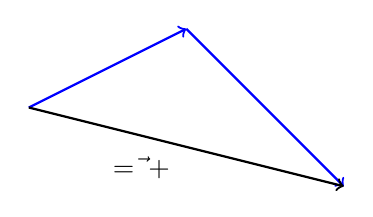
\begin{tikzpicture}
	\draw[->,blue, thick] (-1,1) -- node[above,blue] {$\vect{\matA}$} (1,2);
	\draw[->, blue, thick] (1, 2) --node[above right, blue] {$\vect{\matB}$}  (3, 0);
	\draw[->,thick] (-1, 1) -- node[below left] {$\vect{\matC} = \vec{\matA} + \vect{\matB}$} (3, 0);
	\end{tikzpicture}
\caption{Addition de vecteurs (connue, dans la francophonie, sous le nom de \textit{relation de Chasles}).}
\end{minipage}
\end{figure}


L'ensemble des nombres réels, $\BBR$, peut être représenté par une droite infinie, qu'on
appelle la droite des réels.  Un nombre quelconque $x$ est représenté par
un point sur cette droite.
L'ensemble des couples de nombres réels, $ (x, y) $, peut être représenté par
un point dans un plan.  Ce plan, connu sous  le nom de plan cartésien,
ou $\BBR^2$,
comporte deux axes: l'axe des abscisses (horizontal par convention)  et l'axe des ordonnées (vertical par convention).


Les coordonnées d'un point $(x, y) $ dans ce plan, représentent la distance $x$
du point par rapport à l'axe des ordonnées et sa distance $y$ par rapport à l'axe
des abscisses.  L'intersection des deux axes est l'origine du plan; ses coordonnées
sont $(0, 0)$.

Au lieu de considérer un couple de nombre réels comme un point dans le plan,
on peut considérer qu'il représente un vecteur.  Dans ce cas, chaque coordonnée
représente une \definition{composante} de ce vecteur, $\vect{\matA} = (A_x, A_y)$.\footnote{Une autre
façon d'écrire un vecteur, qui est celle normalement utilisée en algèbre linéaire, 
est en une colonne de composantes: $\vect{\matA} = \displaystyle \binom{ A_x}{A_y}$, c'est-à-dire une matrice
$2\times 1$.}
En utilisant les composantes, l'addition des vecteurs se résume à de simples
addition de nombres:
\begin{eqnarray*}
\vect{\matA} + \vect{\matB} &=& \vect{\matC} \\
(A_x, A_y) + (B_x, B_y) = (A_x + B_x, A_y + B_y) &=& (C_x, C_y)
\end{eqnarray*}
Dans le plan cartésien, on utilise parfois les \definition{vecteurs unitaires}\footnote{Le mot \textit{unitaire} fait référence au 
fait que la grandeur de ces vecteurs est l'unité = 1.} $\iunit = (1, 0)$ et $\junit = (0, 1)$ ce qui nous
permet d'écrire $\vect{\matA} = A_x \iunit + A_y \junit$.

\begin{figure}[h]
\begin{minipage}{0.45\textwidth}
	\begin{tikzpicture}
	% les axes
	\draw[->] (-2,0) -- (2,0) node[anchor=west]{x};
	\draw[->] (0,-2) -- (0,2) node[anchor=south]{y};
	\draw[->,blue] (-2.1, 0.5) node[anchor=south]{\tiny abscisse} -- (-1.7,0);
	\draw[->,blue] (0.8,-1.5) node[anchor=south]{\tiny ordonnée}-- (0,-1.8);
	\draw[->,blue] (-1, -1) node[anchor=north]{\tiny origine (0, 0)} -- (0, 0);
	% le point
	\coordinate [label=right:{(a, b)}] (A) at (1.5, 1);
	\draw[-] (1.5, -0.1) node[anchor=north]{\small a} -- (1.5, 0.1);
	\draw[-] (-0.1, 1) node[anchor=east]{\small b} -- (0.1, 1);
	\draw [dashed, blue] (1.5, 0.2) -- (A);
	\draw [dashed, blue] (0.2, 1) -- (A);
	\fill [black] (A) circle (2pt);
	\end{tikzpicture}
\caption{Un point dans le plan cartésien.}
\end{minipage}\hfill
\begin{minipage}{0.45\textwidth}
	\begin{tikzpicture}
	% les axes
	\draw[->] (-2,0) -- (2,0) node[anchor=west]{x};
	\draw[->] (0,-2) -- (0,2) node[anchor=south]{y};
	\draw[->,thick,blue] (0,0) -- node[anchor=north]{$A_x\iunit$} (1.5, 0);
	\draw[->,thick,blue] (1.5,0) -- node[anchor=west]{$A_y\junit$} (1.5, 1);
	\draw[->,thick] (0,0) -- node[anchor=south]{$\vect{\matA}$} (1.5, 1);
	\end{tikzpicture}
\caption{Un vecteur dans le plan cartésien et sa représentation comme la somme de deux vecteurs
parallèle à chaque axe: les composantes.}
\end{minipage}
\end{figure}
\subsection{Généralisation à $\BBR^n$}
Bien qu'il soit légèrement plus difficile de visualiser des vecteurs dans l'espace que dans le plan, et que ceci deviennent impossible
à faire pour des dimensions égales ou supérieures à 4, il est facile de faire des opérations sur les vecteurs lorsqu'on utilise
les composantes: chaque \definition{dimension} correspond à une valeur de composante, et l'addition de vecteurs
se fait par l'addition de composantes équivalentes, par une simple généralisation de ce qu'on a vu pour deux
dimensions\footnote{Ici on défini la dimension comme étant équivalente au nombre de coordonnées requises pour
identifier un point.  Ainsi, dans le plan, nous avons besoin de deux coordonnées, habituellement dénotées
par $x$ et $y$, pour identifier un point; on dira qu'un plan a deux dimensions.  De la même façon,
une droite a une dimension, et l'espace habituel a trois dimensions.  Un point est un objet ayant zéro dimension.
Plus tard, on verra une autre définition de dimension, lorsqu'on étudiera les espaces vectoriels.}.  
Ceci est en fait un simple cas particulier de l'addition de matrices que nous avons déjà vu.
\textbf{Veuillez prendre note:} à partir d'ici, nous allons presque toujours représenter des vecteurs comme des
matrices colonnes.
%

\section{Les équations linéaires}

Une \definition{équation linéaire} à $n$ variables est une équation de la forme suivante:
\begin{equation}
a_1x_1 + a_2x_2 + \ldots + a_n x_n = b \label{eq:lineaire}
\end{equation}
où les variables $x_1, x_2, \ldots, x_n$ sont les \definition{inconnues} et $a_1, a_2, \ldots, a_n$
sont les \definition{coefficients}.  La variable $b$ est connue sous le nom de \definition{terme constant} de
l'équation linéaire.  On note que l'équation ne compte aucun produit, puissance ou fonction
des \textit{inconnues}.

\begin{exemple}
	Déterminez si les équations suivantes sont linéaires ou non.
	\partexemple{a} $3x_1 - 4x_2 + 5x_3 = 6$
	\partexemple{b} $4x_1 - 5x_2 = x_1 x_2$
	\partexemple{c} $x_2 = 2\sqrt{x_1} - 6$
	\partexemple{d} $x - y = z + \sin 3$
	\partexemple{e} $x_1 + \sin x_2 + x_3 = 1$
	\solution
	\partexemple{a} Oui, car l'équation est de la forme \eqref{eq:lineaire}.
	\partexemple{b} Non, car on a un terme non-linéaire, $x_1 x_2$, qui apparait dans l'équation.
	\partexemple{c} Non, car on a un terme non-linéaire $\sqrt{x_1}$
	\partexemple{d} Oui, car on a trois variables (inconnues) différentes et un terme constant; on peut réécrire
	cette équation comme $x - y - z = \sin 3$ qui est exactement de la forme \eqref{eq:lineaire}.
	\partexemple{e} Non, car on a un terme non-linéaire $\sin x_2$.
\end{exemple}

\begin{exerciceB}
	Déterminez si les équations suivantes sont linéaires ou non.
	\partexercice{a} $x_1^2 + 3x_2 - 2x_3 = 5$
	\partexercice{b} $x_1 + x_1x_2 + 2x_3 = 1$
	\partexercice{c} $x_1 + \displaystyle\frac{1}{x_2} + x_3 = 1$
	\partexercice{d} $5\alpha + 3\beta + 6\gamma = 9$
	\partexercice{e} $x\alpha + y\beta + z\gamma^2 = a^3$
\end{exerciceB}

Une \definition{solution} de l'équation linéaire \eqref{eq:lineaire} est une collection \textbf{ordonnée} de nombres
$s_2, s_2, \ldots, s_n$ qui vérifient  \eqref{eq:lineaire} lorsque $x_i = s_i$ est substitué dans \eqref{eq:lineaire}.
L'ensemble de toutes les solutions d'une équation linéaire s'appelle la \definition{solution générale}.

\begin{exemple}
	Démontrez que $(5 + 4s - 7t, s, t)$, où $s, t \in\BBR$, est une solution de l'équation
	\[
	x_1 - 4x_2 + 7x_3 = 5
	\]
	\solution
	En substituant $x_1 = 5+4s - 7t, x_2=s$ et $x_3=t$ on obtient
	\[
	x_1 - 4x_2 + 7x_3 =
	\underbrace{5+4s-7t}_{x_1} - 4s+ 7t = 5
	\]
	ce qui est le résultat désiré.
	\end{exemple}
	Les variables $s$ et $t$ de l'exemple précédent sont connues sous le nom de \definition{paramètres},
	et on dit que la solution est exprimée dans une \definition{forme paramétrique}.

	Une équation linéaire peut avoir soit une solution, une infinité de solution, ou aucune solution.
	\begin{exemple}
	Déterminez le nombre de solutions pour chacune de ces équations.
	\partexemple{a} $0x = 5$
	\partexemple{b} $2x = 4$
	\partexemple{c} $x - 4y = 8$
	\solution
	\partexemple{a} Puisque le côté gauche de cette équation est 0, et que le côté droit est 5, cette équation n'a aucune solution.
	\partexemple{b} On peut vérifier facilement que $x=2$ est l'unique solution de cette équation.
	\partexemple{c} Si on attribue la valeur arbitraire $s$ à $y$, on peut vérifier que $x= 8 - 4s$ sera une solution de cette équation.
	Comme $s$ peut prendre une infinité de valeurs différentes, cette équation a une infinité de solutions.
\end{exemple}
%

\begin{exemple}
	Montrez que si $x_1+kx_2 = c$ et $x_1 + \ell x_2 = d$ sont des équations équivalentes, alors on doit avoir
	$k = \ell$ et $c=d$.
	\solution
	Comme on a une équation avec deux inconnues, on écrit la solution de la première équation sous une
	forme paramétrique avec la
	paire ordonnée, $(c-kt, t)$ --- la valeur de $t$ étant totalement arbitraire.  En substituant ces valeurs
	dans la deuxième équation, on trouve
	$
	(c-kt) + \ell t = d.
	$
	En choisissant $t=0$, on trouve que $c=d$.  En substituant cette valeur, on trouve le résultat désiré.
\end{exemple}

%%%%%%%%%%%%%%%%%%%%%%%%%%%%%%%%%%%%%%%%%%%%%%%%%%%
\section{Systèmes d'équations linéaires}
%%%%%%%%%%%%%%%%%%%%%%%%%%%%%%%%%%%%%%%%%%%%%%%%%%%

Un \definition{système d'équations linéaires} est un ensemble de plusieurs équations linéaires
qui sont satisfaites simultanément.

\subsection{Exemple trivial}
Soit le système de deux équations linéaires%
\footnote{Dans un système d'équations linéaires, chaque ligne contient une seule équation.
Pour des raisons qui deviendront plus claires dans les prochains chapitre, nous allons
utiliser le mot ligne plutôt que le mot équation pour identifier une équation individuelle.}:
\[
\left\{ \begin{matrix}
    x &=& 1 \\
    y &=& 2
    \end{matrix}
    \right.
\]
On obtient un système d'équations équivalentes, c'est-à-dire qu'il admet la même
solution $(x=1, y=2)$ si on écrit les
lignes dans un ordre différent:
\[
 L_1  \leftrightarrow L_2 \Rightarrow
\left\{ \begin{matrix}
    y &=& 2 \\
    x &=& 1
    \end{matrix}
    \right.
\]
On obtient un système d'équations équivalentes si on multiplie une des lignes par une constante différente
de zéro
\[
3L_1 \rightarrow L_1 \Rightarrow \left\{ \begin{matrix}
    3y &=& 6 \\
    x &=& 1
    \end{matrix}
    \right.
\]
On obtient un autre système d'équations équivalentes si on multiplie une des lignes par une constante différente
de zéro et qu'on y ajoute une autre ligne:
\begin{equation}\label{eq:triv}
L_1 + 4L_2 \rightarrow L_1 \Rightarrow \left\{ \begin{matrix}
    3y &+& 4x &=& 10 \\
    && x &=& 1
    \end{matrix}
    \right.
\end{equation}
\begin{exerciceB}
Vérifiez que $(x=1, y=2)$ est toujours une solution de l'équation \eqref{eq:triv}.
\end{exerciceB}
Ces manipulations sur les lignes d'un système d'équations linéaires sont appelées
\definition{opérations élémentaires sur les lignes}; nous les reverrons en détails
dans les prochains chapitre.  En utilisant ce type de manipulation, on peut
facilement résoudre les systèmes d'équations linéaires.
\begin{exemple}
	Trouvez la solution générale du système d'équations linéaires suivant:
	\[
	\left\{\begin{matrix}
	x_1 &+& x_2 &=& 7 \\
	2x_1 &+& 4x_2 &=& 18
	\end{matrix}
	\right.
	\]
	\solution
	En multipliant la première équation par -2 et en additionnant le résultat à
	la deuxième équation comme suit:
	\[
	-2L_1 + L_2 \rightarrow L2 \Rightarrow \left\{\begin{matrix}
	x_1 &+& x_2 &=& 7 \\
	&& 2x_2 &=& 4
	\end{matrix}
	\right.
	\]	
  on trouve que $2x_2 = 4$, et donc $x_2=2$.
	En substituant ceci dans la première équation, on trouve que $x_1=5$
\end{exemple}

\begin{exerciceB}
	Trouvez la solution générale du système d'équations linéaires suivant:
	\[
	\left\{\begin{matrix}
	x_1 &+& 2x_2 &=& 8 \\
	3x_1 &-& x_2 &=& 4
	\end{matrix}
	\right.
	\]
\end{exerciceB}

\begin{exemple}
	En faisant le choix $x_3 = t$ avec $t$ un paramètre arbitraire, trouvez la
	solution générale du système d'équations linéaires suivant:
	\[
	\left\{\begin{matrix}
	x_1 &+& x_2 &+& x_3 &=& 7 \\
	2x_1 &+& 4x_2  &+& x_3 &=& 18
	\end{matrix}
	\right.
	\]
	\solution
	Avec le choix $x_3 = t$, on peut récrire le système d'équations linéaires sous la forme
		\[
	\left\{\begin{matrix}
	x_1 &+& x_2 &=& 7 -t \\
	2x_1 &+& 4x_2 &=& 18-t
	\end{matrix}
	\right.
	\]
	En multipliant la première équation par -2 et en additionnant le résultat à
	la deuxième équation comme suit
			\[
	-2L_1 + L_2 \rightarrow L_2 \Rightarrow \left\{\begin{matrix}
	x_1 &+& x_2 &=& 7 -t \\
	&& 2x_2 &=& 4 + t
	\end{matrix}
	\right.
	\]
	 on trouve que $2x_2 = 4 + t$, et donc $ x_2= 2 + \frac{1}{2}t$.
	En substituant ceci dans la première équation, on trouve que $x_1=5 - \frac{3}{2}t$
\end{exemple}

\begin{exerciceB}
	En faisant le choix $x_3 = t$ avec $t$ un paramètre arbitraire, trouvez la
	solution générale du système d'équations linéaires suivant:
	\[
	\left\{\begin{matrix}
	x_1 &+& 2x_2 &+& x_3 &=& 8 \\
	3x_1 &-& x_2 &+& x_3 &=& 4
	\end{matrix}
	\right.
	\]
\end{exerciceB}


%%%%%%%%%%%%%%%%%%%%%%%%%%%%%%%%%%%%%%%%%%%%%%%%%%%
\section{Systèmes d'équations linéaires: quatre interprétations}
Soit le système d'équations linéaires suivant:
\begin{equation}
\left\{
\begin{matrix}
x &+&2y &=& 4 \\
x &-& y &=& 1 
\end{matrix}
\right.\label{eq:interp4}
\end{equation}
On peut vérifier facilement que la solution unique est donnée par
$x=2, y=1$.
Ce système, tout simple, peut être interprété de quatre façons comme nous
allons le voir ci-dessous.  Ces interprétations donnent un tout petit aperçu
des domaines d'utilisation de l'algèbre linéaire et de certains sujets que
nous allons couvrir.

\begin{marginfigure}
\includegraphics[width=1.8in]{images/descartes.jpg}
\caption{René Descartes, 1596--1650.  Mathématicien, physicien et philosophe français, 
d'après qui l'on nomme le plan cartésien.}\label{image:descartes}
\end{marginfigure}

\subsection{Interprétation géométrique}
Dans un premier temps, le système \eqref{eq:interp4} peut être vu comme
deux équations de droites dans le plan cartésien.
La solution correspond au point d'intersection des deux droites.  Si les deux
droites sont parallèles (mais non confondues), il n'y a pas de point d'intersection
et le système n'a pas de solutions.  Si les deux droites sont confondues, alors
il existe une infinité de solutions.

\begin{figure}[h]
\begin{minipage}{0.45\textwidth}
	\begin{tikzpicture}
	% les axes
	\draw[->] (-1,0) -- (5,0) node[anchor=west]{\color{gray}x};
	\draw[->] (0,-1) -- (0,5) node[anchor=south]{\color{gray}y};
	% les deux droites
	\draw[-, thick, blue] (0,-1) -- (5,4) node[anchor=east]{\color{blue}\small $x-y=1$};
	\draw[-, thick, purple] (-1,2.5) node[anchor= south west]{\color{purple}\small $x+2y=4$}  --(5,-0.5);
	% le point d'intersection
	\coordinate (A) at (2,1);
	\draw[-] (2, -0.1) node[anchor=north]{\small 2} -- (2, 0.1);
	\draw[-] (-0.1, 1) node[anchor=east]{\small 1} -- (0.1, 1);
	\draw [dashed, gray] (2, 0.2) -- (A);
	\draw [dashed, gray] (0.2, 1) -- (A);
	\end{tikzpicture}
\caption{L'intersection des deux droites représente la solution unique du système d'équations.}
\end{minipage}\hfill
\begin{minipage}{0.45\textwidth}
	\begin{tikzpicture}
	% les axes
	\draw[->] (-1,0) -- (5,0) node[anchor=west]{\color{gray}x};
	\draw[->] (0,-1) -- (0,5) node[anchor=south]{\color{gray}y};
	% les deux droites
	\draw[-, thick, purple] (-1,2.5) -- node[anchor= south west]{\color{purple}\small $x+2y=4$} (5,-0.5);
	\draw[-, thick, blue] (-1,4) -- node[anchor= south west]{\color{blue}\small $x+2y=6$} (5,1);
	\end{tikzpicture}
\caption{Un système à deux inconnues sans solution: les deux droites sont parallèles. À noter qu'on pourrait
avoir une infinité de solutions si les deux droites étaient confondues.}\label{fig:parallel}
\end{minipage}
\end{figure}

Si on ajoute une inconnue, pour passer de deux à trois, alors chaque équation linéaire représente
un plan dans l'espace.  Si on a trois équations, on aura alors trois plans.  Si ces trois plans s'intersectent
en un seul point, alors il y aura une solution unique.  Si deux plans sont parallèles, il n'y aura aucune
solution.  Il peut également n'y avoir aucune solutions si les plans s'intersectent deux à deux, le long de droites,
mais si ces droites sont parallèles entre elles.  On peut également avoir une infinité de solutions, si les trois
plans s'intersectent le long d'une droite commune.
\begin{figure}[h]
\begin{minipage}{0.3\textwidth}
\includegraphics[width=1.8in]{images/three-planes-1.jpg}
\caption{Intersection de trois plan avec un point commun aux trois.}
\end{minipage}
\hfill
\begin{minipage}{0.3\textwidth}
\includegraphics[width=1.8in]{images/three-planes-0.jpg}
\caption{Intersection de trois plan sans point commun: deux plans sont parallèles.}
\end{minipage}
\hfill
\begin{minipage}{0.3\textwidth}
\includegraphics[width=1.8in]{images/three-planes-2.jpg}
\caption{Intersection de trois plan sans point commun: les plans s'intersectent deux à deux, mais
les trois droites ainsi formées sont colinéaires.}
\end{minipage}
\end{figure}

%
\begin{marginfigure}
\includegraphics[width=1.8in]{images/plane_intersect.png}
\caption{Jeu de mots anglais sur l'intersection des plans (origine de l'image inconnue).}
\end{marginfigure}
%

%
\subsection{Équation matricielle} 
Il est facile de vérifier que le système d'équations linéaires \eqref{eq:interp4} peut être écrit sous
forme matricielle comme suit:
\[
\begin{pmatrix}
1 & 2 \\
1 & -1
\end{pmatrix}
\begin{pmatrix}
x \\ y
\end{pmatrix}
=
\begin{pmatrix}
4 \\
1
\end{pmatrix}
\]
Avec les choix
\[
\matA = \begin{pmatrix}
1 & 2 \\
1 & -1
\end{pmatrix}, \qquad \matX=
\begin{pmatrix}
x \\ y
\end{pmatrix}
, \qquad
\matB = 
\begin{pmatrix}
4 \\
1
\end{pmatrix}
\]
on obtient une équation toute simple: $\matA \matX = \matB$.  Si on pouvait diviser une matrice par une autre, on serait tenté d'écrire que la solution serait:
\[
\matX = \frac{\matB}{\matA}
\]
Cependant, on ne peut pas faire ceci car la division par une matrice n'est pas une opération définie.
Par contre, on peut \textbf{parfois} définir un \textit{inverse multiplicatif} défini par la relation
$\matA^{-1}\matA=\matI$. Lorsque c'est le cas\footnote{Nous verrons les conditions pour l'existence d'un
tel inverse plus tard.}, on peut alors écrire la solution comme
\[
\matX = \matA^{-1}\matB
\]
tout comme si les matrices étaient de simples nombres.

%
\subsection{Combinaison linéaire}
\notation{combinaison linéaire}
%
Une autre façon d'écrire le système d'équations linéaires \eqref{eq:interp4} est la suivante:
\[
x \binom{1}{1}+ y\binom{2}{-1} = \binom{4}{1}
\]
Si on définit les vecteurs $\vect{A}, \vect{B}$ et $\vect{C}$ de la façon suivante:
\[
\vect{A}= \binom{1}{1}, \qquad \vect{B}=\binom{2}{-1}, \qquad \vect{C} = \binom{4}{1}
\]
on peut alors récrire l'équation sous la forme
\[
x\vect{A} + y\vect{B} = \vect{C}
\]

\begin{figure}[h]
\begin{center}
	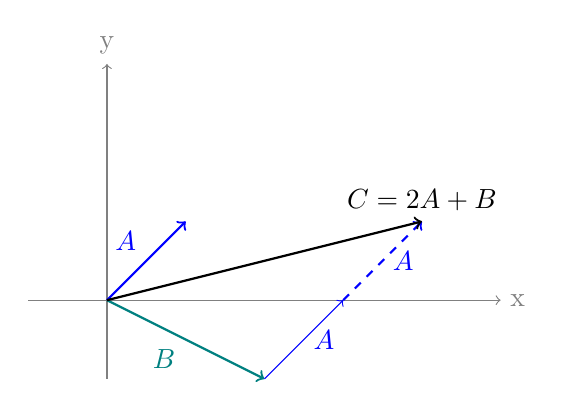
\begin{tikzpicture}
	% les axes
	\draw[->, gray] (-1,0) -- (5,0) node[anchor=west]{\color{gray}x};
	\draw[->, gray] (0,-1) -- (0,3) node[anchor=south]{\color{gray}y};	
	%
	\draw[->,blue, thick] (0,0) -- node[above left,blue] {$\vect{A}$} (1,1);
	\draw[->, teal, thick] (0,0) -- node[below left, teal] {$\vect{B}$}  (2,-1);
	\draw[->, blue] (2,-1) -- node[right,blue] {$\vect{A}$} (3,0);
	\draw[->, blue, dashed, thick] (3,0) -- node[right,blue] {$\vect{A}$}(4,1);
	\draw[->,thick] (0,0) --  (4,1) node[above] {$\vect{C} = 2\vect{A} + \vect{B}$};
	\end{tikzpicture}
\caption{Combinaison linéaire de vecteurs}
\end{center}
\end{figure}

On a donc une somme vectorielle avec deux inconnues.  
Ce type de somme de vecteurs s'appelle une combinaison linéaire.
Un exemple plus abstrait est donné en chimie par la méthode de combinaison linéaire d'orbitales atomiques.
Les combinaisons linéaires sont la base de l'étude des \definition{espaces vectoriels} que nous verrons plus tard.

\subsection{Transformation linéaire}
Une quatrième interprétation est possible en considérant l'équation sous forme matricielle
\[
\matA \matX = \matB
\]
Selon cette interprétation, la matrice $\matA$ effectue des transformations sur des vecteurs d'un domaine initial pour les transformer dans un domaine connu sous le nom d'image de la transformation.  
Un exemple de telles transformations est celui des rotations dans le plan, où le domaine initial et celui de l'image sont identiques.  
Un exemple différent est celui d'une projection: pour chaque point aux coordonnées $(x, y, z)$, on fait sa projection dans le plan $xy$.  Dans ce cas-ci, le domaine initial est $\BBR^3$; celui de l'image est $\BBR^2$. 
Sous forme d'équation matricielle, on écrirait une 
telle projection de la façon suivante:
\[
\begin{pmatrix}
1 & 0 & 0 \\
0 & 1 & 0
\end{pmatrix}
\begin{pmatrix}
x\\y\\z
\end{pmatrix}
=
\begin{pmatrix}
x\\y
\end{pmatrix}
\]
Plusieurs autres exemples existent tel que nous le verrons plus tard.  Mais auparavant, nous devons étudier un peu plus à fond les équations linéaires et les matrices.
